Na teoria das elei��es, o M�todo de Borda sugere que, em vez de escolher um candidato, cada juiz deve criar um ranking de sua prefer�ncia para os concorrentes (isto �, criar uma lista com a ordem de classifica��o dos concorrentes). A este ranking � associada uma pontua��o: um ponto para o �ltimo colocado no ranking, dois pontos para o pen�ltimo, tr�s para o antepen�ltimo, e assim sucessivamente. Ao final, soma-se a pontua��o atribu�da a cada concorrente por cada um dos ju�zes. 
Em uma escola houve um concurso de poesia no qual cinco alunos concorreram a um pr�mio, sendo julgados por 25 ju�zes. Para a escolha da poesia vencedora foi utilizado o M�todo de Borda. Nos quadros, est�o apresentados os rankings dos ju�zes e a frequ�ncia de cada ranking. 

\begin{figure}[h]
\centering
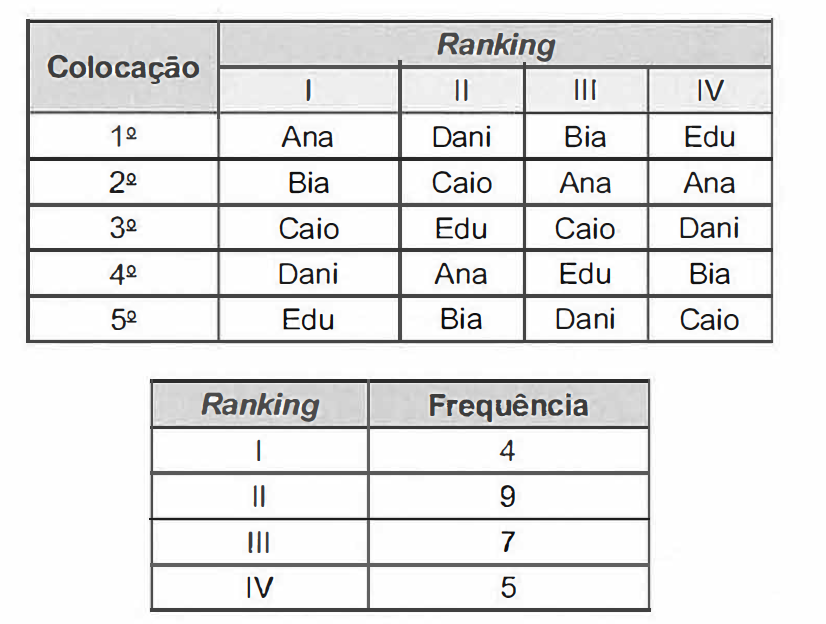
\includegraphics[width=8cm]{../figuras/q141-2018.png}
\end{figure}

\begin{enumerate}
\item[a)]Edu.
\item[b)]Dani.
\item[c)]Caio.
\item[d)]Bia
\item[e)]Ana.
\end{enumerate}